\section{外掛程式}

\begin{frame}{麥卡托投影}
\only<8>{
\begin{center}
{\fontsize{150pt}{50pt}\selectfont 厚}

\includegraphics[width=5cm]{penguin.jpeg}
\end{center}
}\only<1-7,9->{
\begin{multicols}{2}
\begin{itemize}
\item 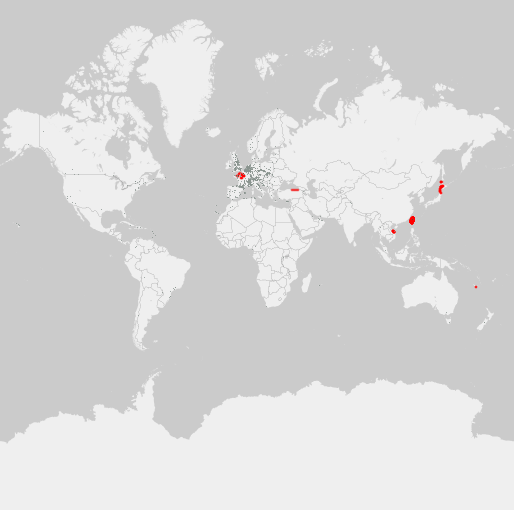
\includegraphics[width=4cm]{worldMap.png}
\pause
\item 放大$\frac1{\cos(\text{緯度})}$倍
\pause
\item 特性:小範圍內的地圖方位、比例尺都是對的
\pause
\item 活動距離通常不會太遠 $\then$ 麥卡托投影(除非你搭飛機還開 Strava )
\pause
\newpage
\item Q: 麥卡托投影有辦法畫出整個地球嗎?
\pause
\item A: 沒辦法,所以去南極探險開 Strava 不會紀錄在地圖上
\pause
\item 企鵝表示:
\pause
\pause
\item 假設赤道畫在地圖上的寬度是$2\pi r$,那畫到南北緯$\theta$的地圖的高度就是$2r\ln|\sec\theta+\tan\theta|$,所以正方形的地圖會畫到南北緯$\tan^{-1}\left(\frac12(e^\pi+e^{-\pi})\right)\approx85.07$度。\\
{\tiny $\int_0^\theta\frac1{\cos x}dx=\left.\ln|\sec x+\tan x|\right|_0^\theta=\ln|\sec\theta+\tan\theta|$}
\end{itemize}
\end{multicols}
}
\end{frame}

\begin{frame}{Statshunter}
\only<1-2>{
\begin{multicols}{2}
\begin{itemize}
\item 網頁:\url{https://www.statshunters.com}

\includegraphics[width=3cm]{QRcodeStats.png}\pause
\item Heatmap:所有騎過的路線畫出的地圖
\end{itemize}
\newpage
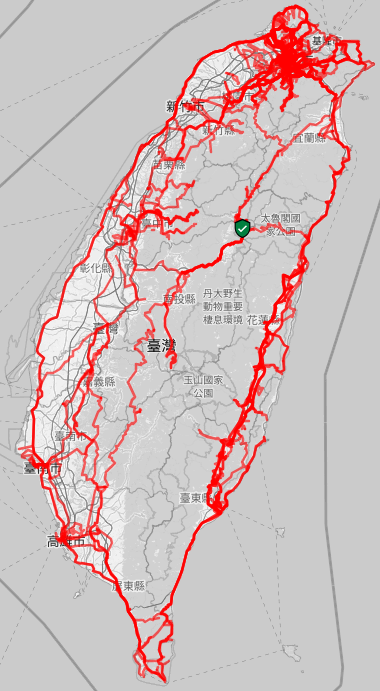
\includegraphics[height=6.5cm]{statsTaiwan.png}
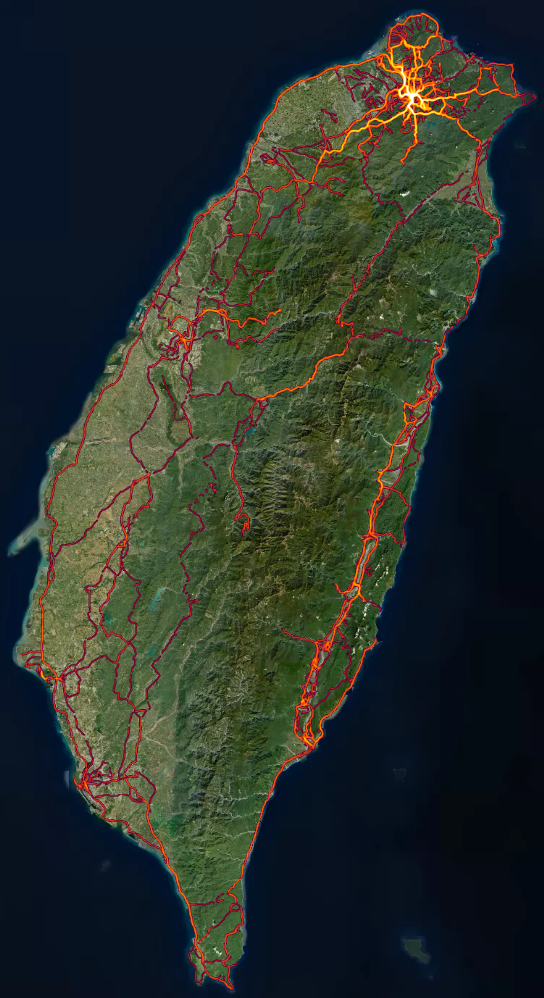
\includegraphics[height=6.5cm]{taiwanHeatmap.png}
\end{multicols}
}\only<3>{
\begin{itemize}
\item Explore tiles:Statshunter 會把整個世界地圖切成$2^{14}\times2^{14}$個(近似)正方形的格子\\
格子的寬度$=$赤道長度$\times\cos($緯度$)\times2^{-14}\approx2.446\times\cos($緯度$)km$\\
\item 在台北一格大約是$2.217km\times2.217km$,而在奧克蘭一格大約是$1.957km\times1.957km$
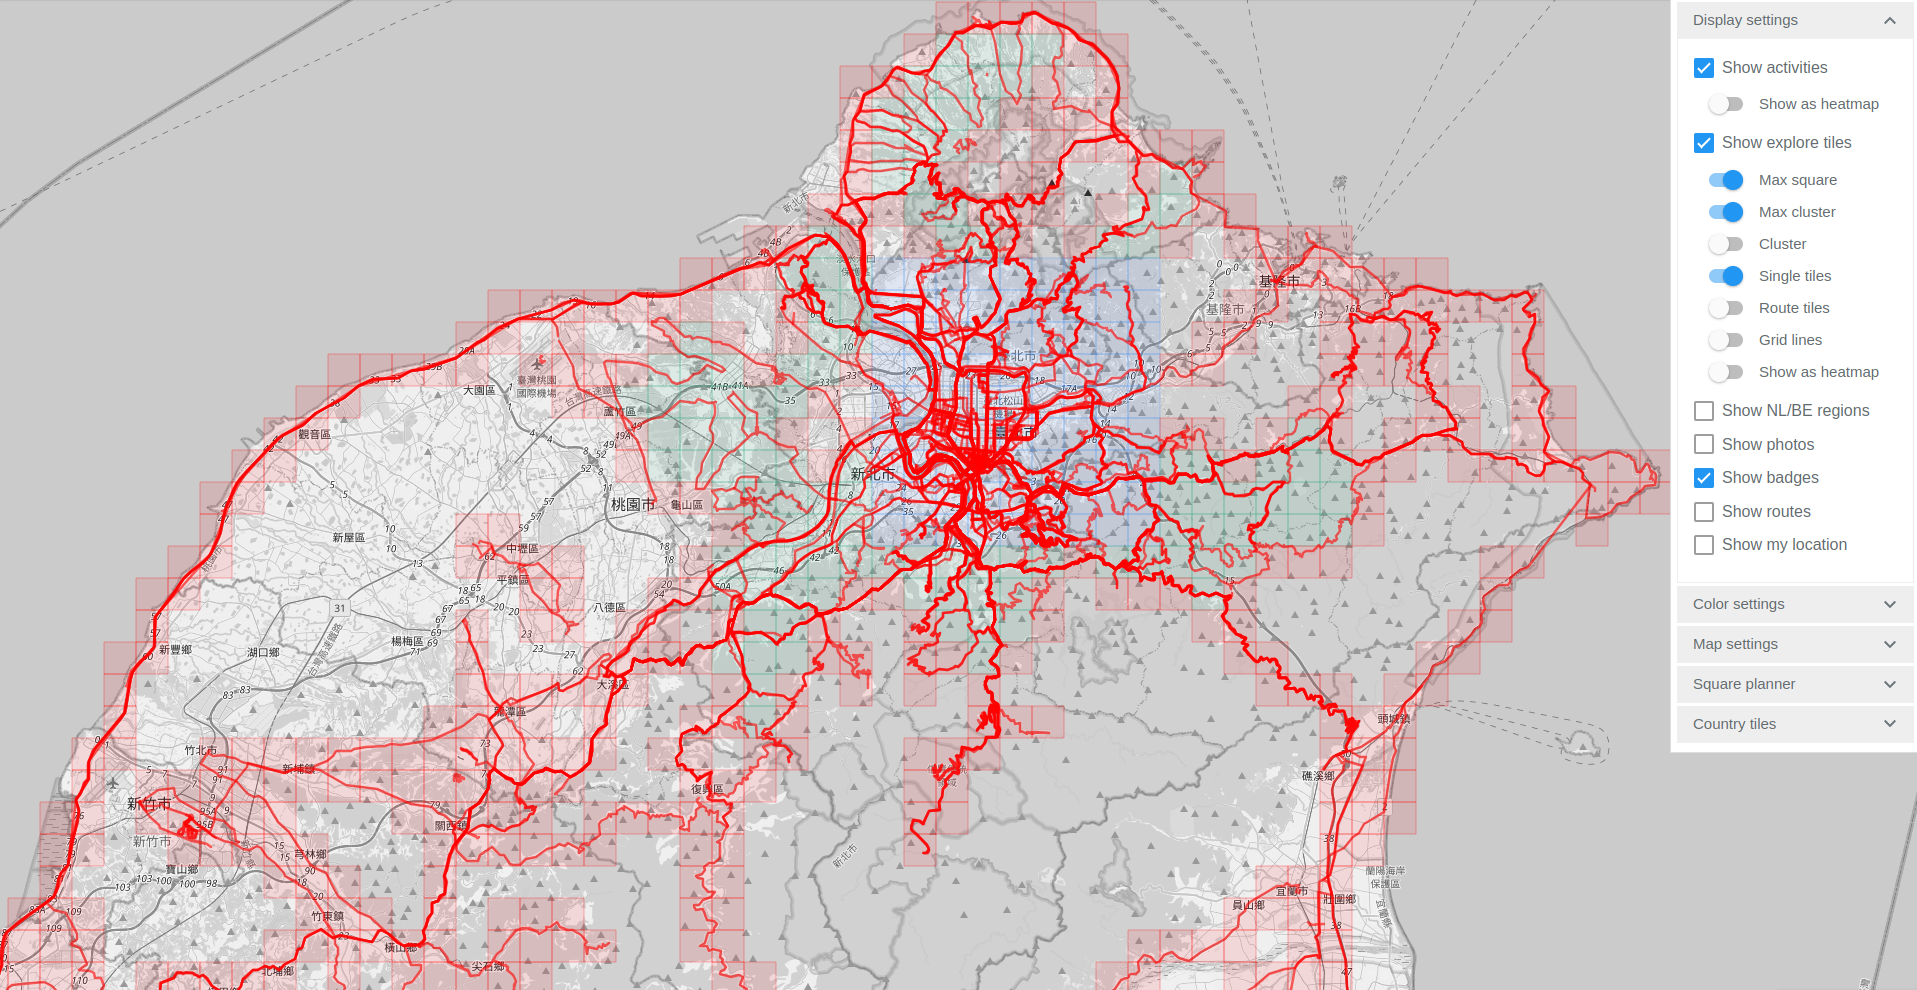
\includegraphics[width=11cm]{statsTaipei.png}
\end{itemize}
}\only<4-7>{
\pause\pause\pause
\begin{multicols}{2}
\begin{itemize}
\item Filter:比如說你可能只想看某段時間內的 heatmap 、統計數據\\\pause
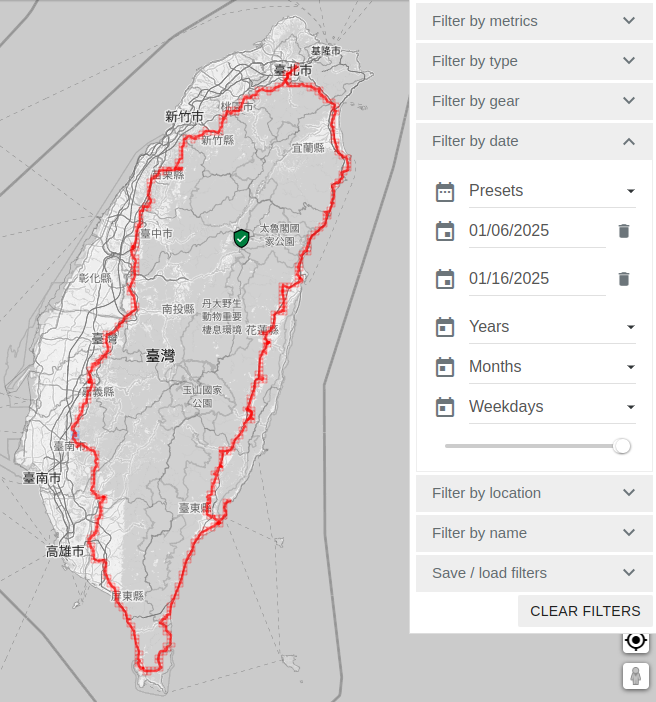
\includegraphics[height=4.5cm]{filterTaiwan.png}\pause
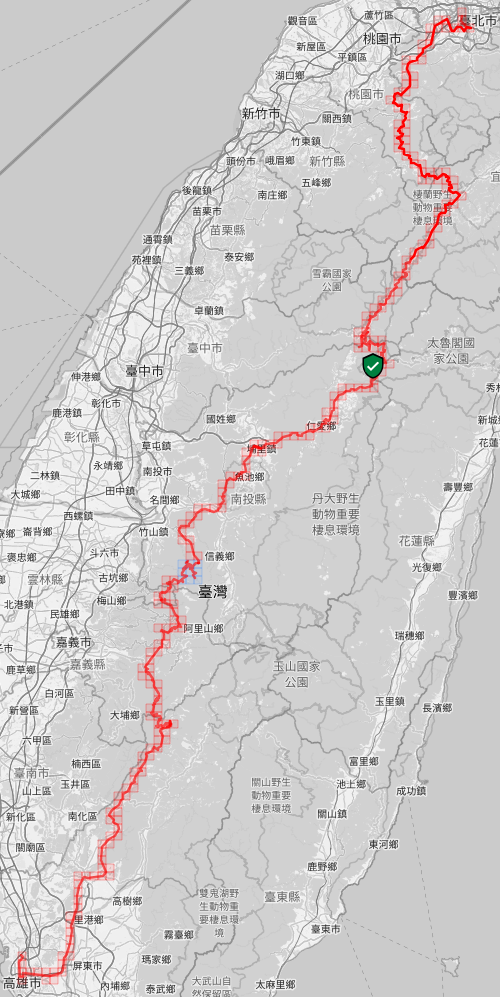
\includegraphics[height=4.5cm]{filterRoof.png}
\end{itemize}
\newpage\pause
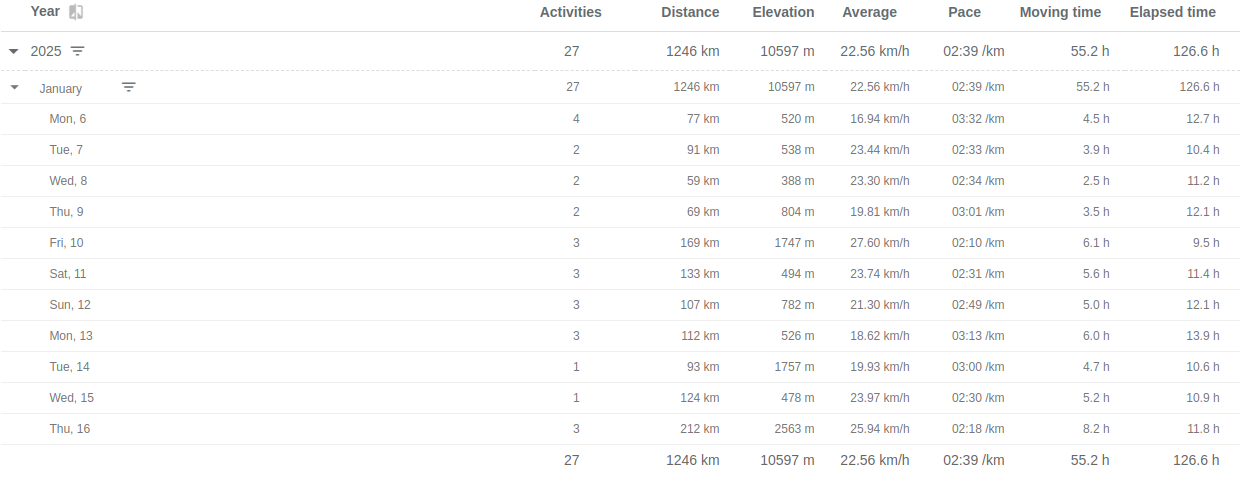
\includegraphics[width=7cm]{filterTaiwanStats.png}
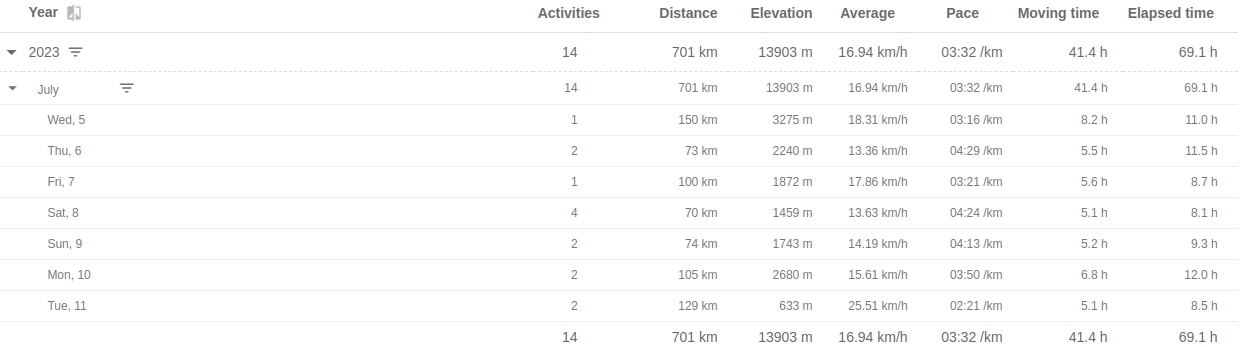
\includegraphics[width=7cm]{filterRoofStats.png}
\end{multicols}
}\only<8-9>{
\pause\pause\pause\pause\pause\pause\pause
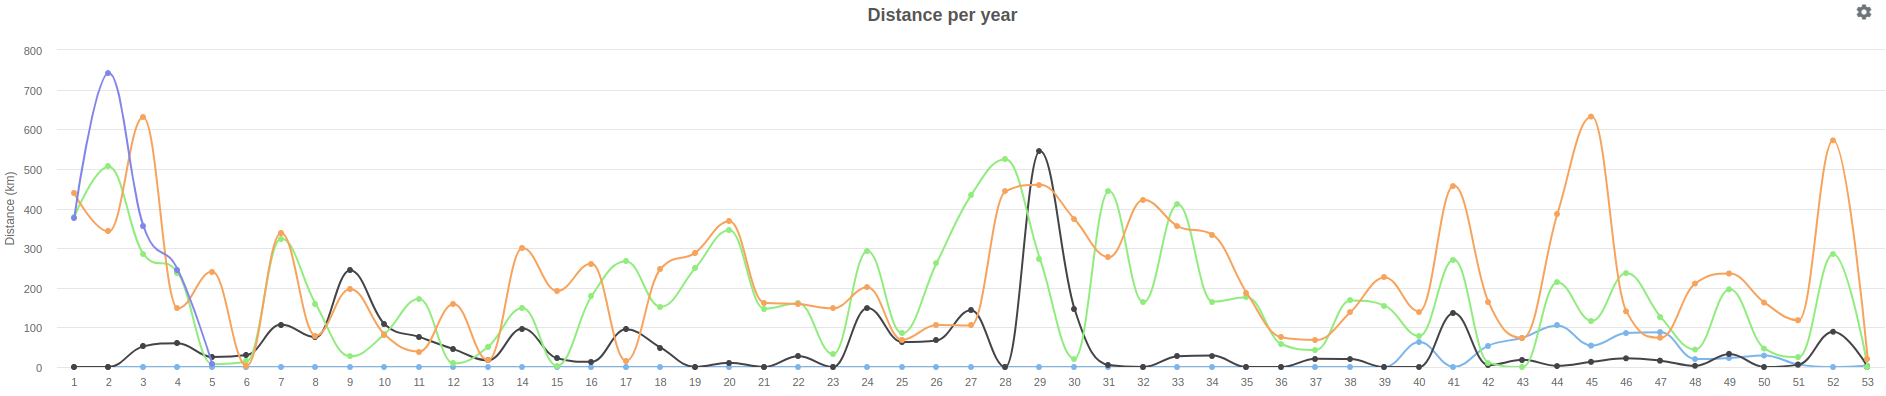
\includegraphics[width=15cm]{statsDistance.png}\\\pause
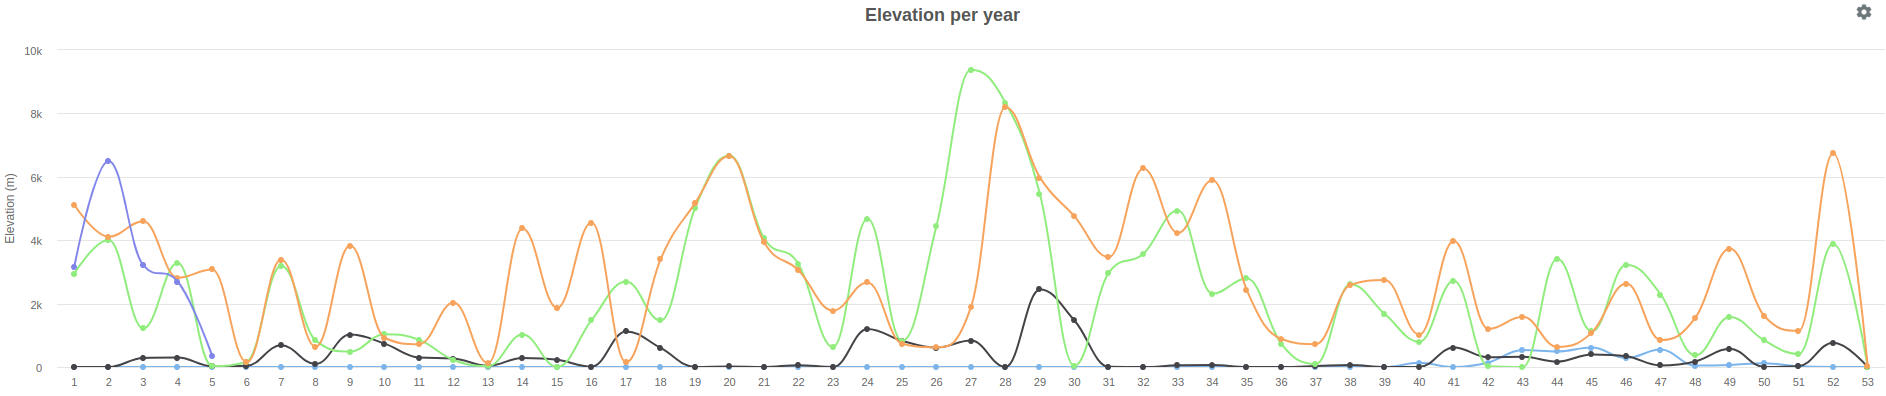
\includegraphics[width=15cm]{statsElevation.png}
}\only<10-11>{
\pause\pause\pause\pause\pause\pause\pause\pause\pause
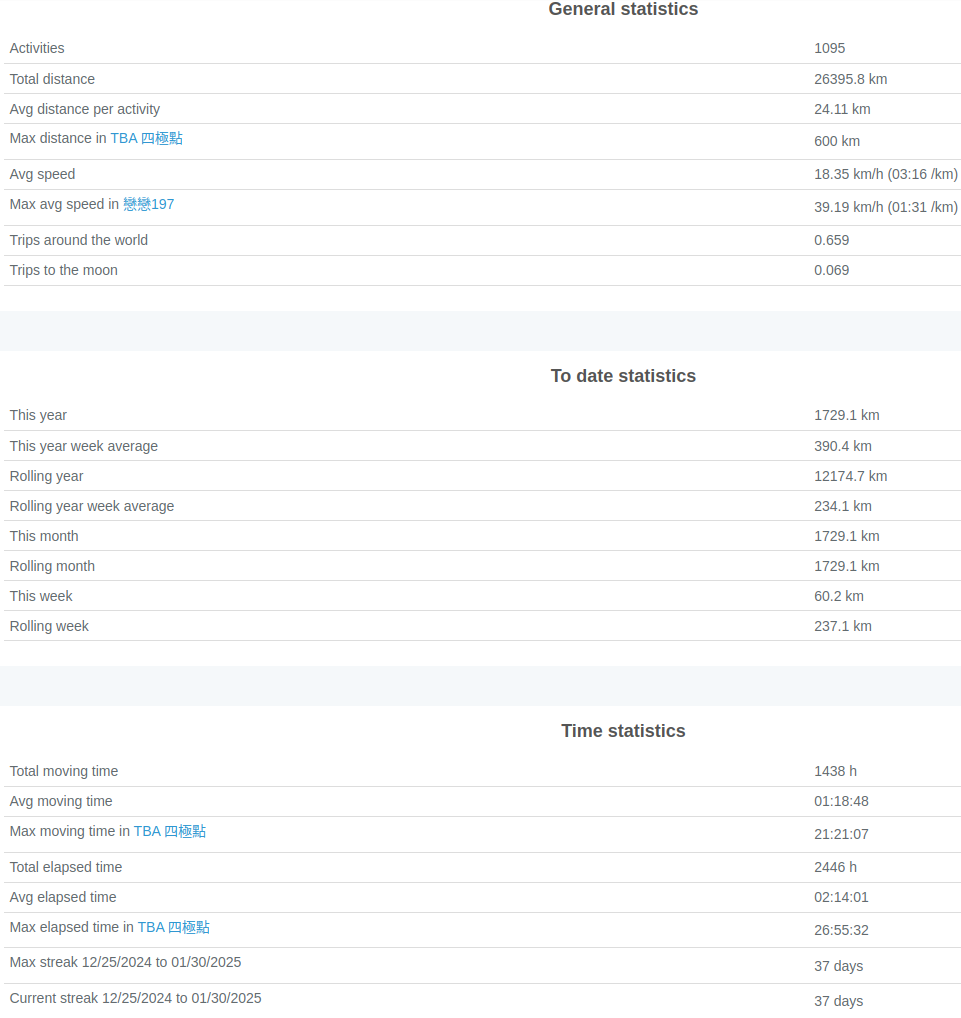
\includegraphics[height=7cm]{statsAll.png}\pause
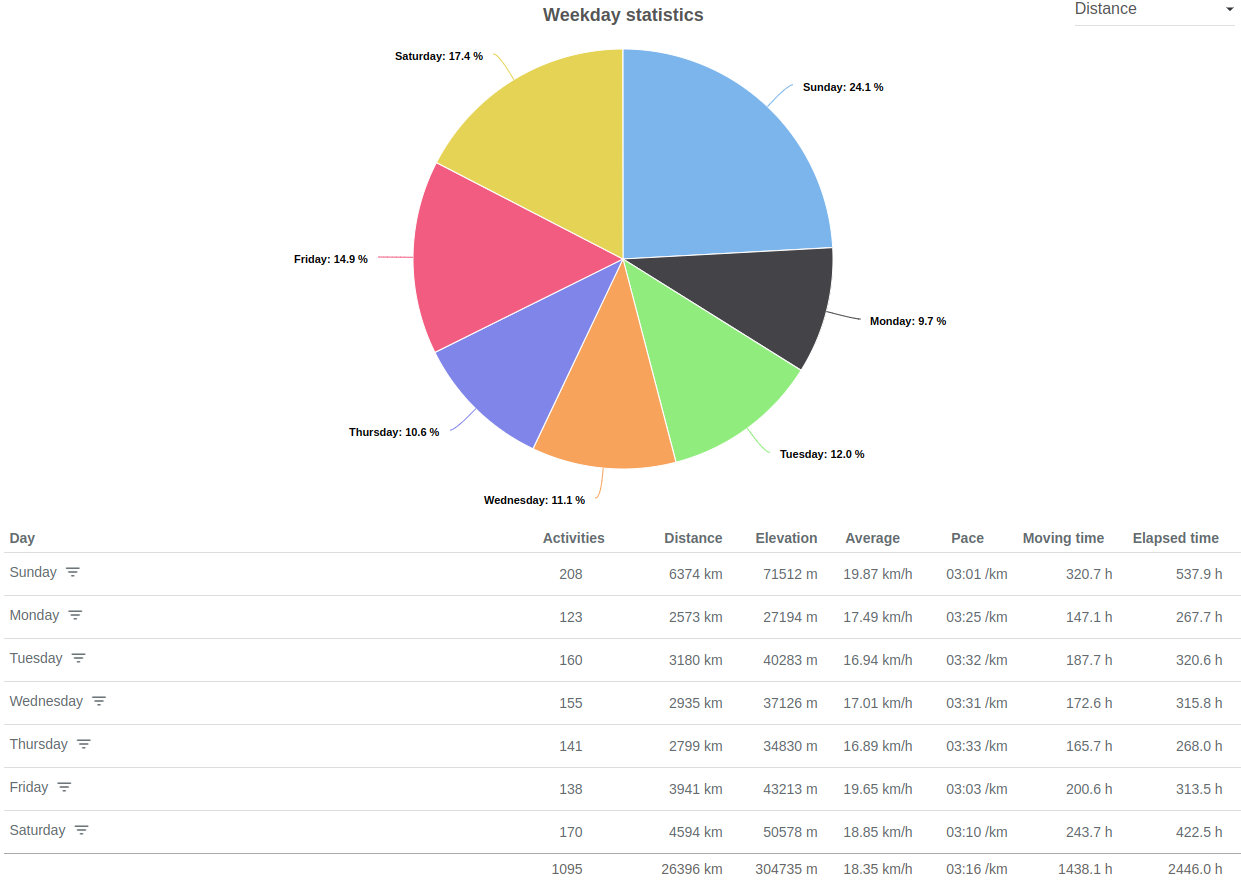
\includegraphics[height=6cm]{statsWeek.png}
}\only<12-13>{
\pause\pause\pause\pause\pause\pause\pause\pause\pause\pause\pause
\includegraphics[width=7.5cm]{statshour.png}\pause
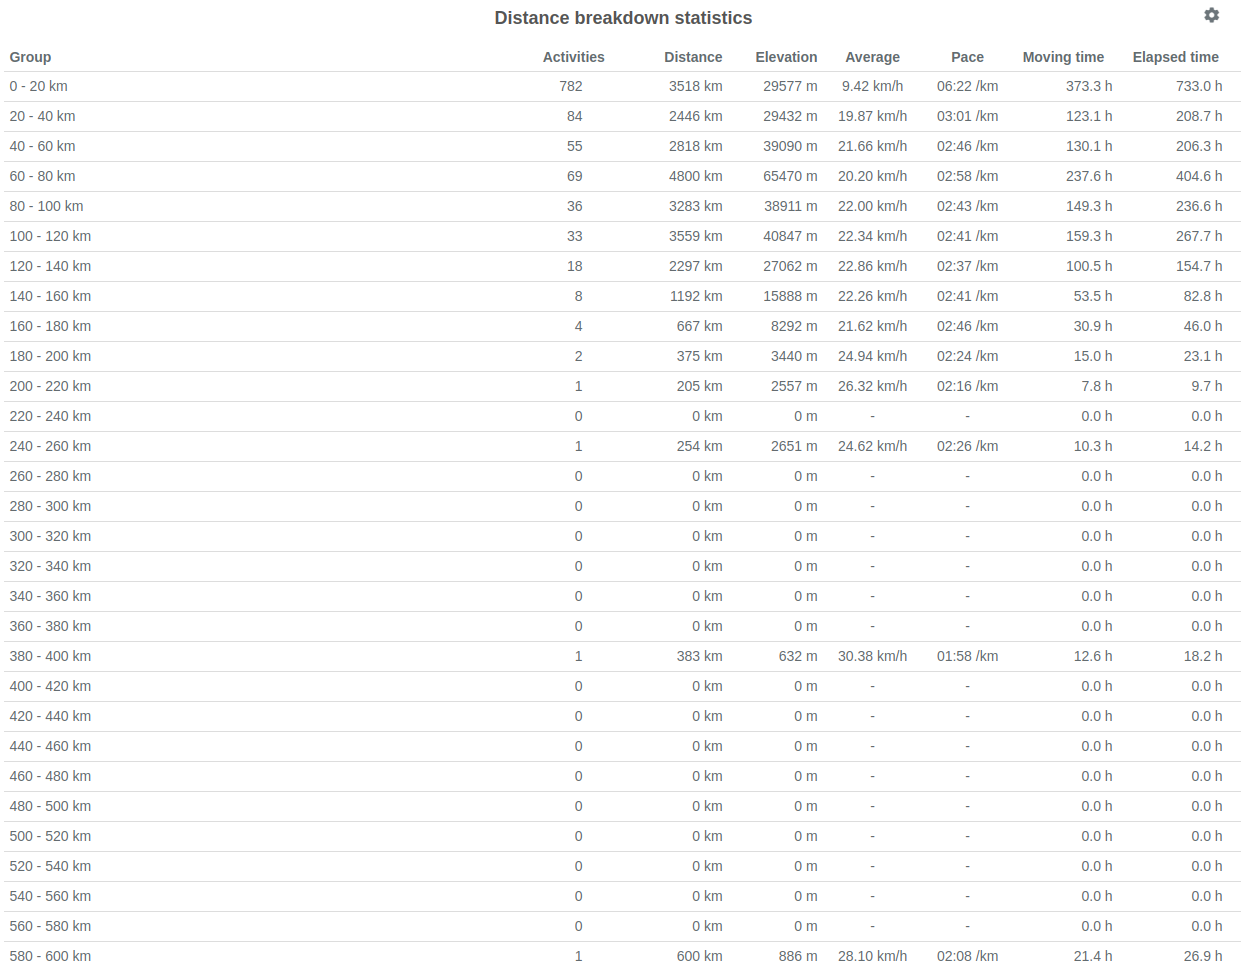
\includegraphics[width=7.5cm]{distanceBreakdown.png}
}\only<14->{
\pause\pause\pause\pause\pause\pause\pause\pause\pause\pause\pause\pause\pause
\begin{multicols}{2}
\begin{itemize}
\item 分享 Statshunter :點選左上角三條線 $\to$Share$\to$ADD SHARE\\
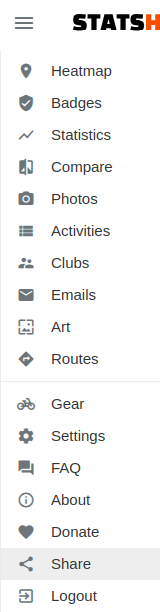
\includegraphics[height=4cm]{share1.png}\\

\includegraphics[width=5cm]{share2.png}\pause
\newpage
\item 勾選要分享的資料\\
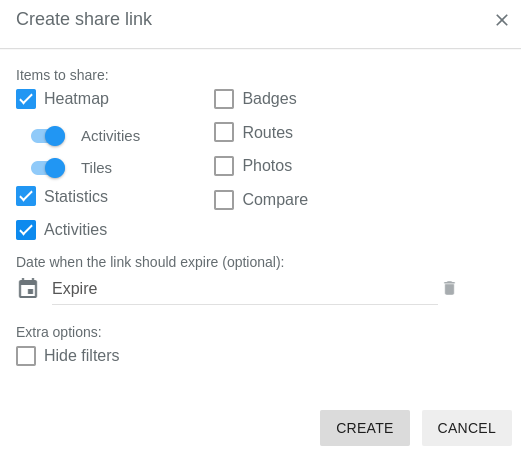
\includegraphics[width=3.5cm]{share3.png}\pause
\item 然後就可以把產生的連結傳給別人了\\

\includegraphics[width=3cm]{share4.png}
\end{itemize}
\end{multicols}{2}
}
\end{frame}

\begin{frame}[fragile]{Flyby}
\only<1>{
\begin{itemize}
\item 打開方法:設定$\to$隱私控管功能$\to$Flyby$\to$所有人\\
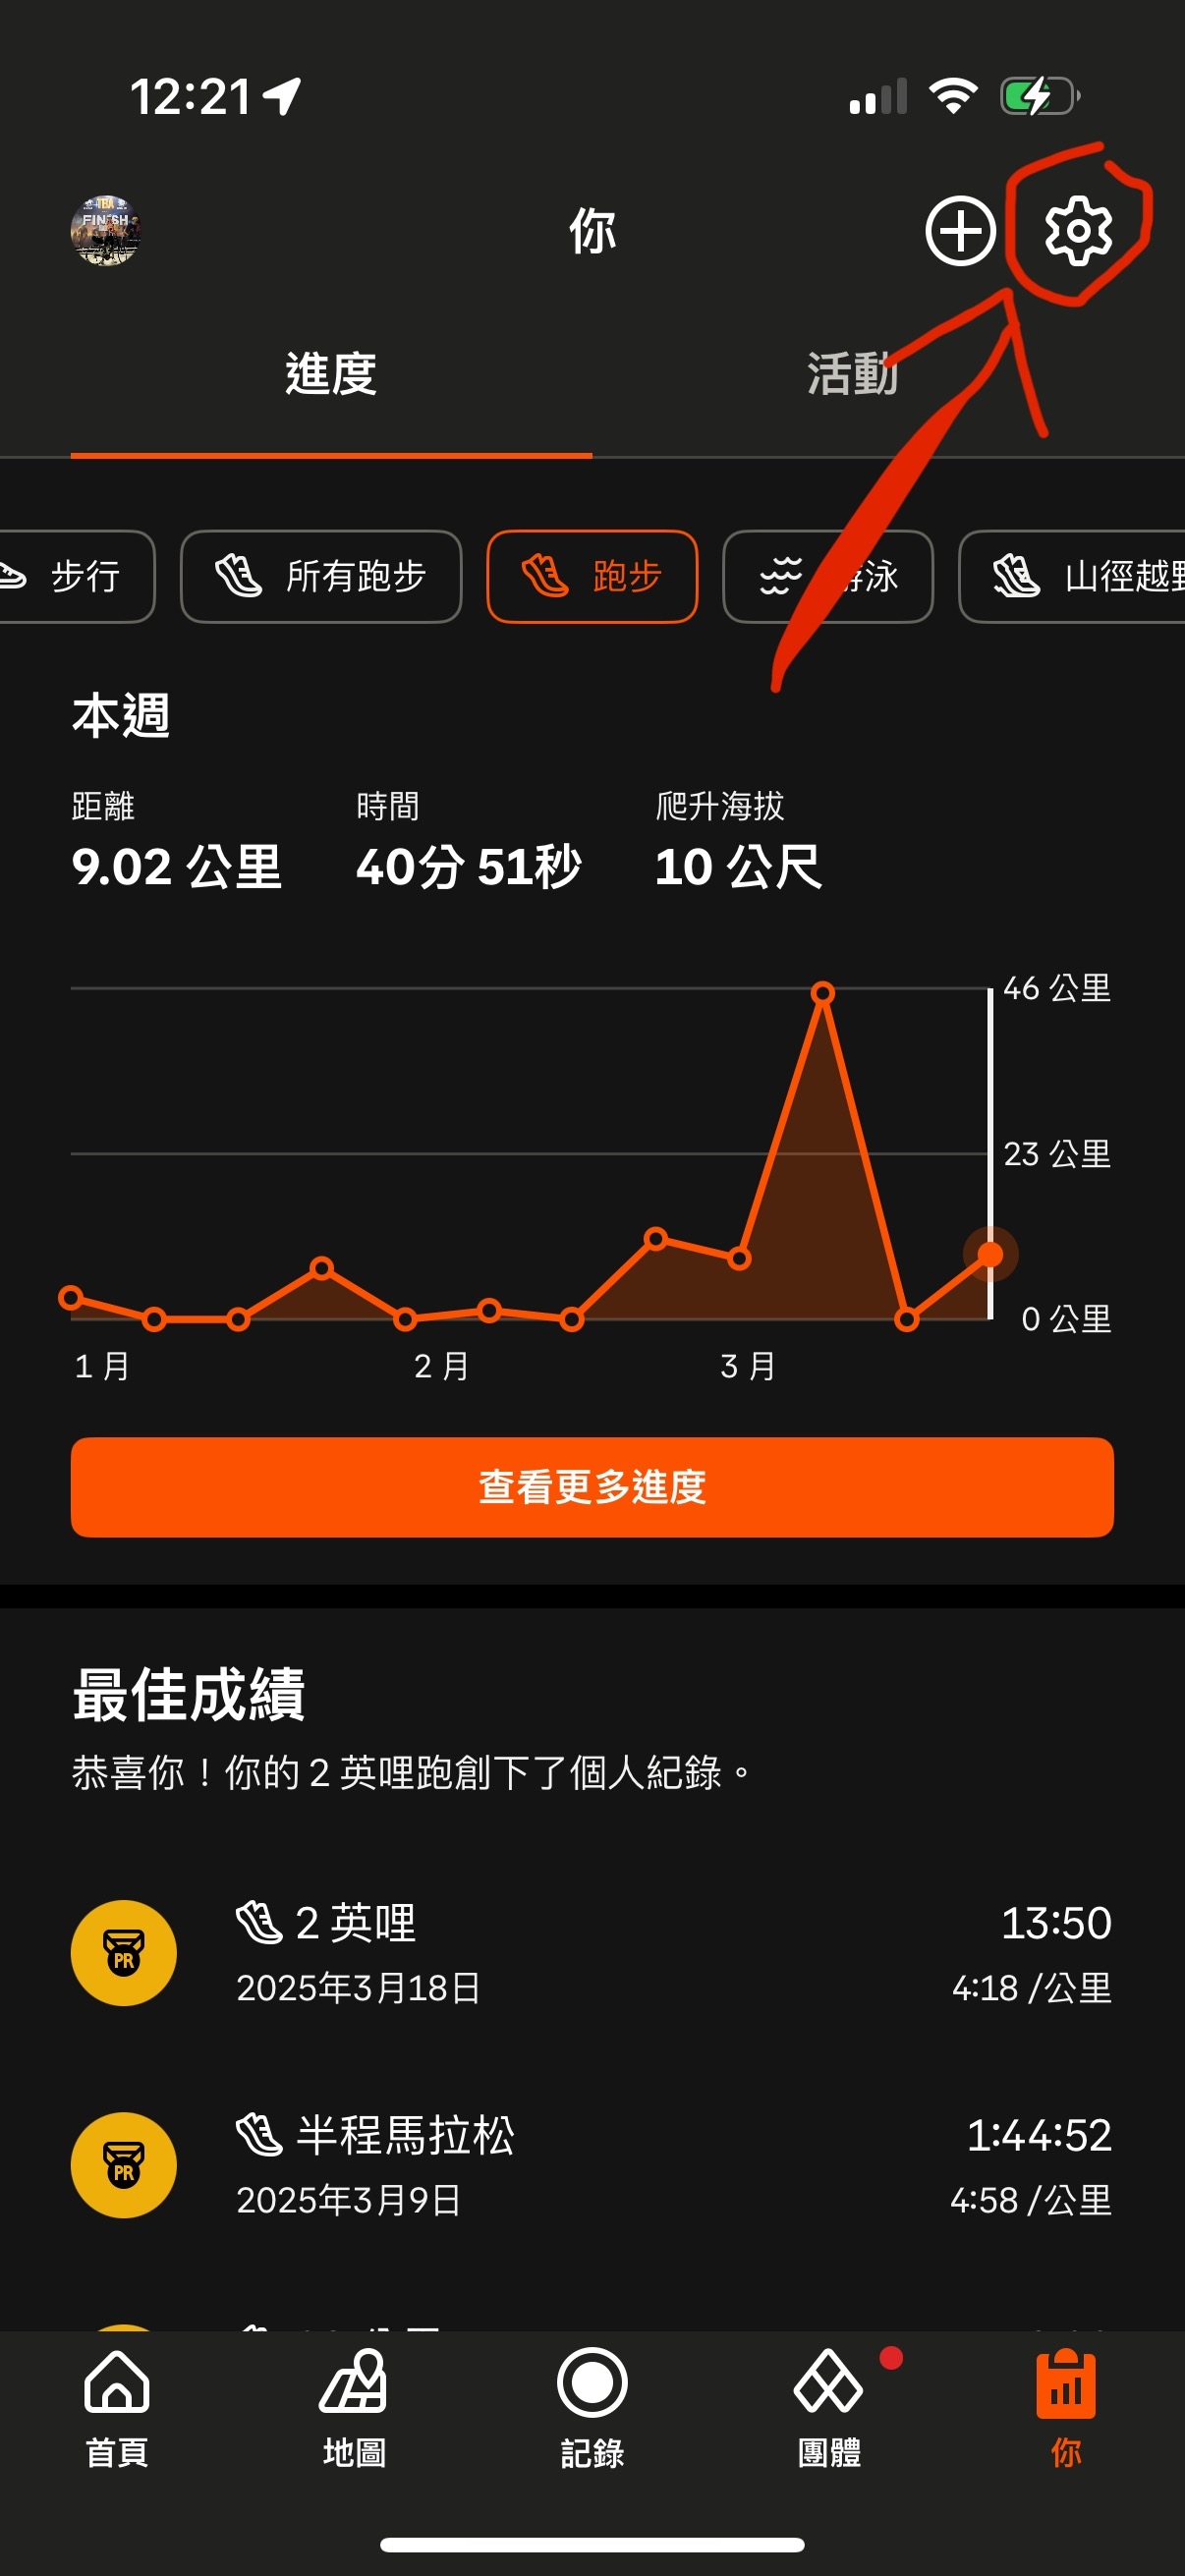
\includegraphics[height=6cm]{openFlyby1.png}

\includegraphics[height=6cm]{openFlyby2.png}
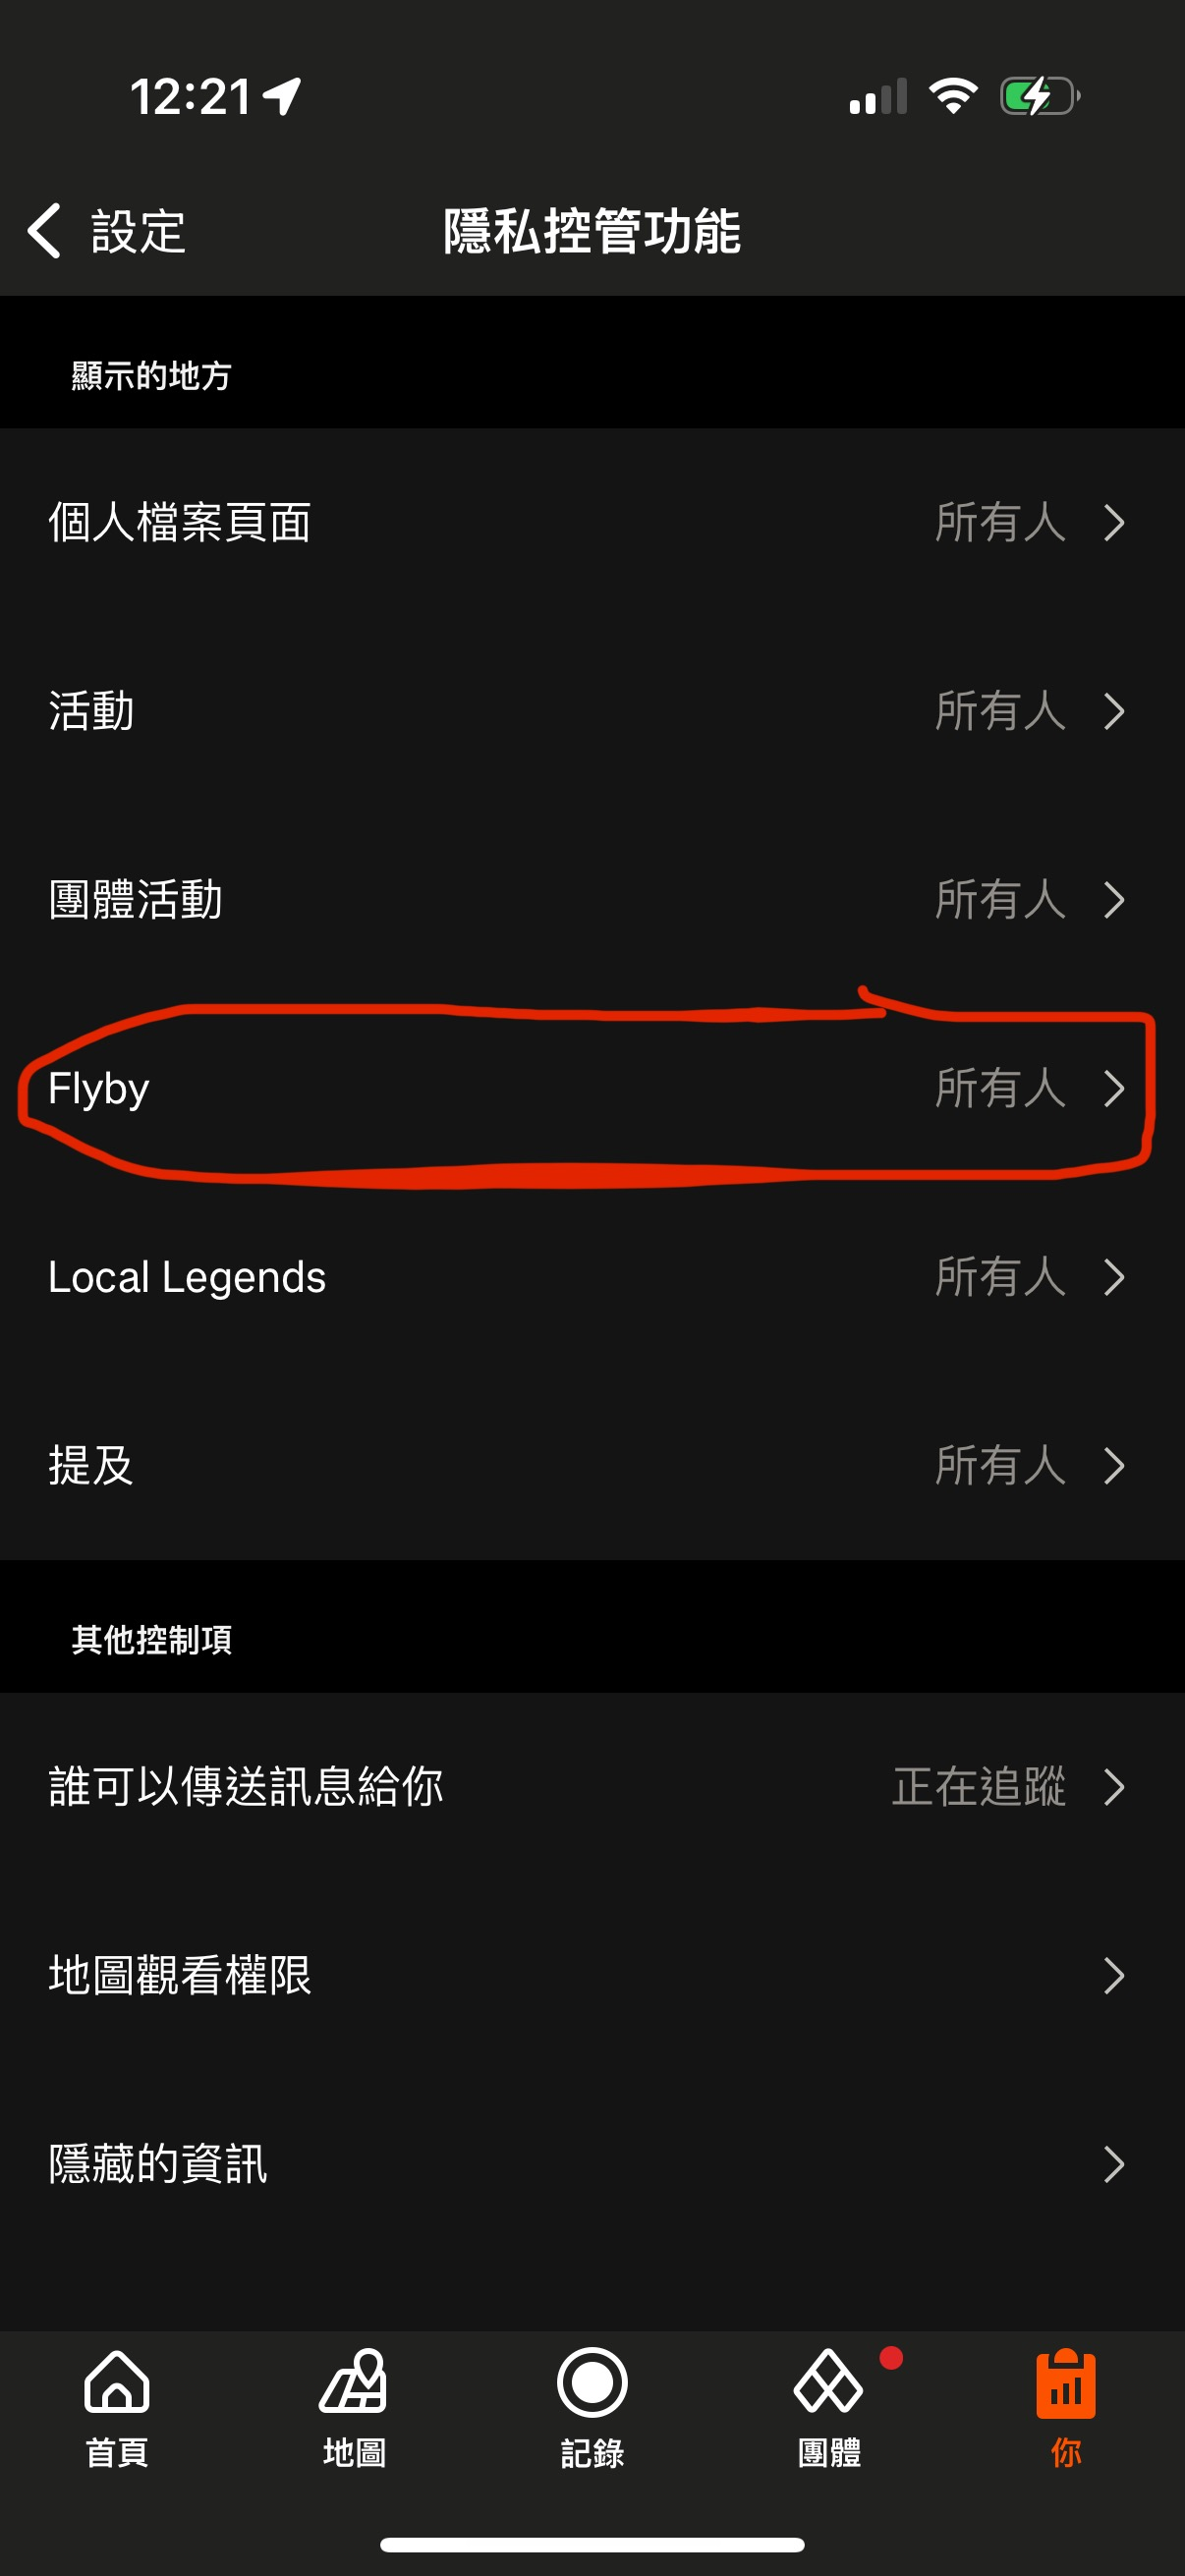
\includegraphics[height=6cm]{openFlyby3.png}

\includegraphics[height=6cm]{openFlyby4.png}
\end{itemize}
}\only<2>{
\begin{itemize}
\item 用上帝視角看在某個特定時間點所有的人分別在哪裡
\item 比對每個人的領先/落後的狀況
\item 檢視單個活動的 \href{https://labs.strava.com/flyby/viewer/\#12860322097}{Flyby} (需使用網頁版):\\

\includegraphics[height=5cm]{openFlyby.png}

\includegraphics[height=5cm]{flybyQRCode.png}
\end{itemize}
}
\only<3>{
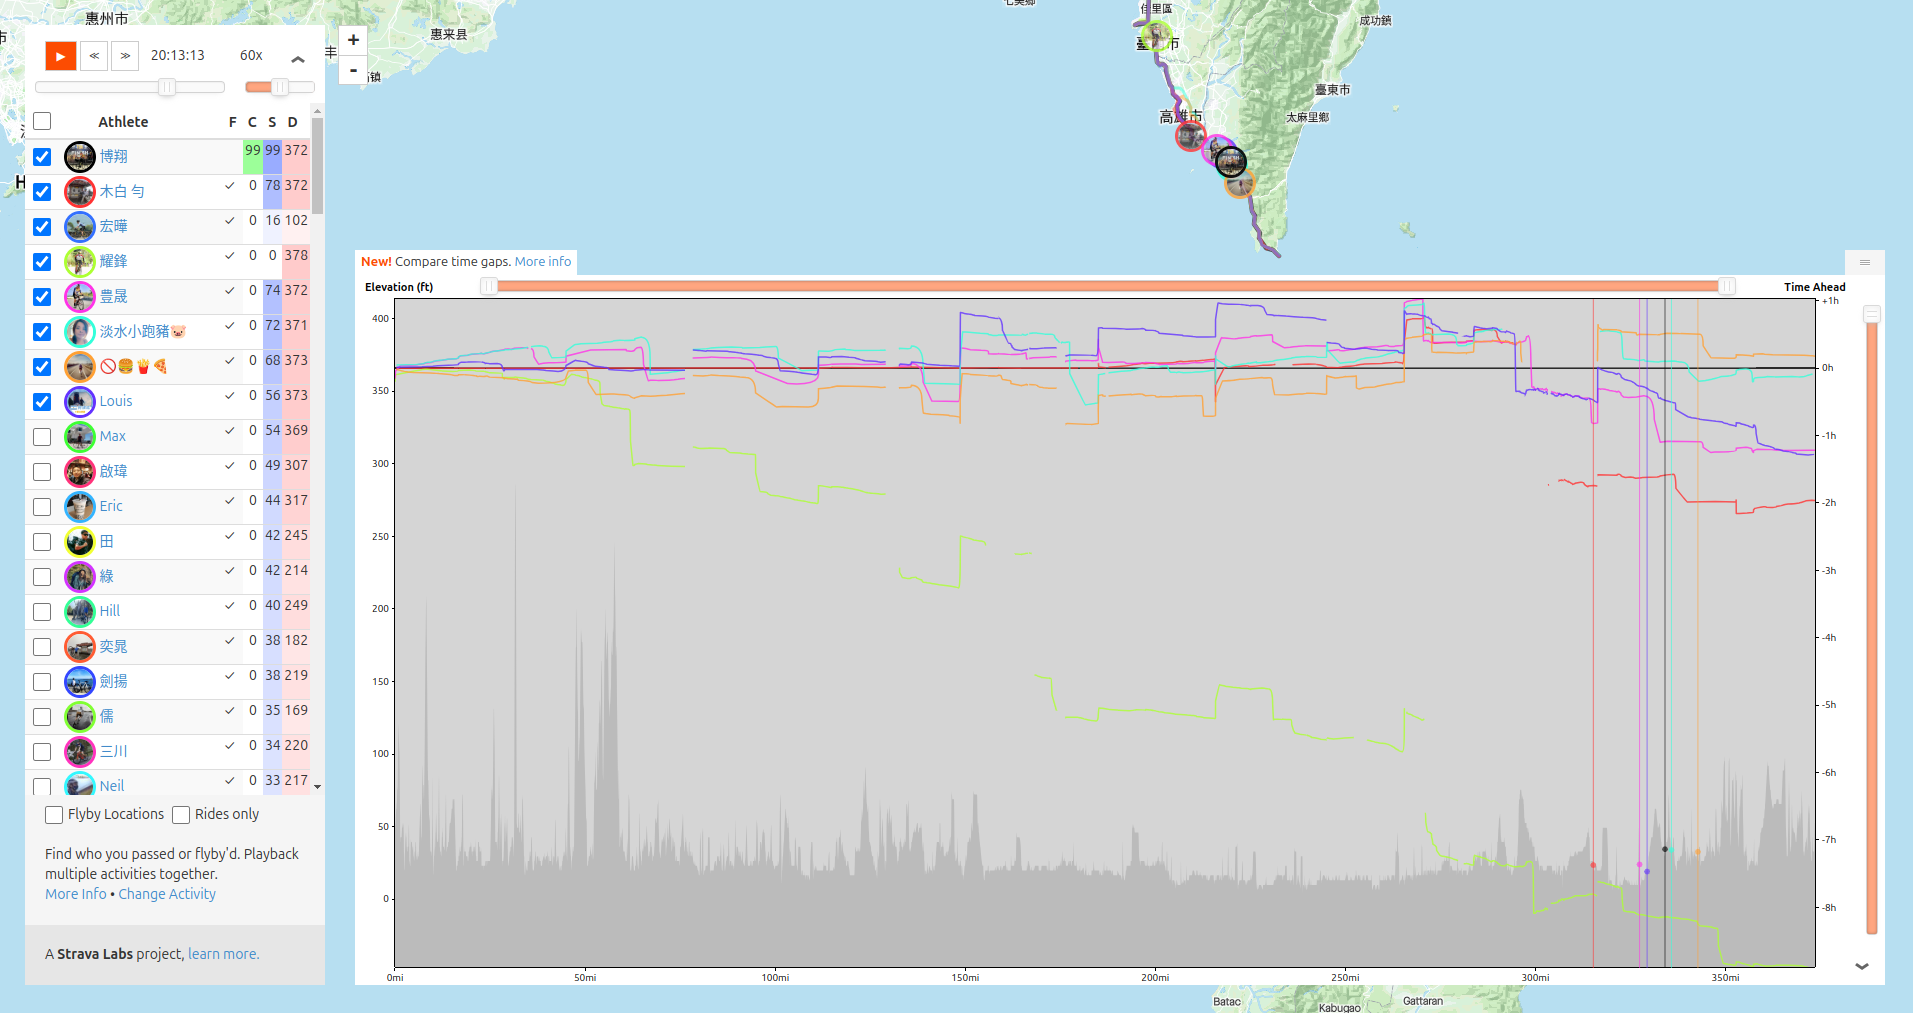
\includegraphics[width=15cm]{flyby.png}
}
\end{frame}

\begin{frame}{Intervals}
\begin{itemize}
\only<2>{
\item 分析訓練強度
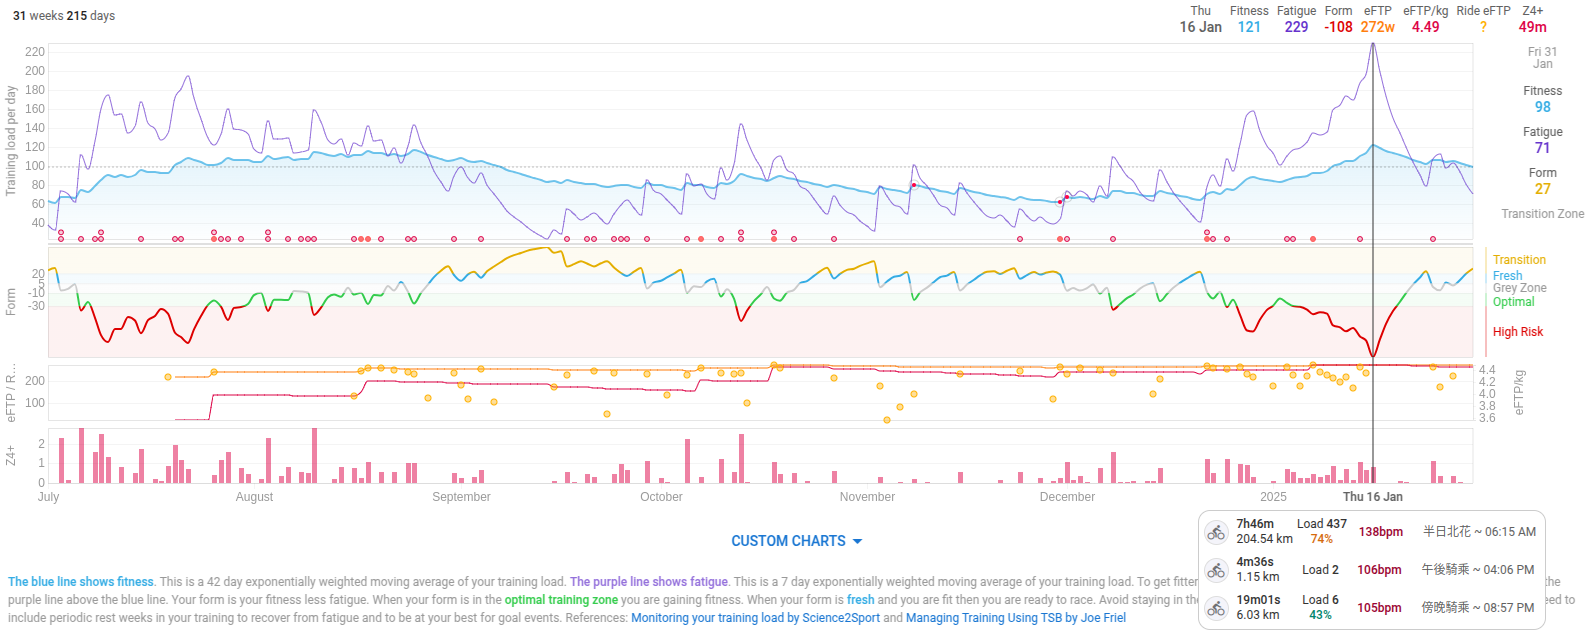
\includegraphics[width=14cm]{intervalsFitness.png}
}\only<1>{
\item 分析功率、心率資料
\item 估計FTP
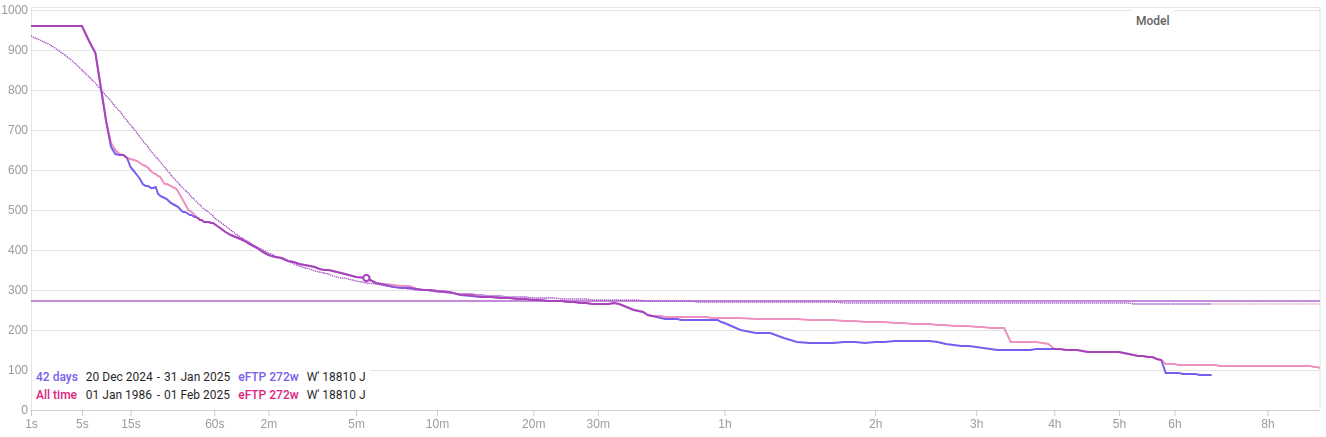
\includegraphics[width=14cm]{intervalsPower.png}
}
\end{itemize}
\end{frame}

